%begin---------------------Settings---------------------------%
\documentclass[12pt,a4paper,UTF8]{article}
\usepackage{geometry}
	\geometry{left=2cm,right=2cm,top=3.2cm,bottom=2.8cm}
\usepackage{amsmath,paralist,enumitem,booktabs,multirow,graphicx,subfig,setspace,listings,lastpage}
\usepackage[colorlinks,
            linkcolor=blue,       
            anchorcolor=blue,  
            citecolor=blue,       
            ]{hyperref}
	\setlength{\parindent}{2em}
	\lstset{language=Python}
\usepackage{fancyhdr}
	\pagestyle{fancy}
	\lhead{C6}
	\rhead{SUPPLEMENTARY INFORMATION}
	\cfoot{Page \thepage/\pageref{LastPage}}
	\rfoot{\today}
	\renewcommand{\headrulewidth}{0.4pt}
	\renewcommand{\theenumi}{(\arabic{enumi})}

\renewcommand{\thefigure}{S\arabic{figure}}
\renewcommand{\thetable}{S\arabic{table}}


%%begin-----------------Reference-----------------------%%
\usepackage[hyperref=true,backend=biber,bibstyle=gb7714-2015,citestyle=numeric-comp,sorting=none,backref=true]{biblatex}
\addbibresource{REF.bib}
%%end-------------------Reference-----------------------%%

%end---------------------Settings---------------------------%



%%%%%%%%%%%%%%%%%%%%%%%%%%%%%%%%%%%%%%%%%%%%%%%%%%%%%%%%%%
%%%%%%%%%%%%%%%%%%%%%%%%%Document%%%%%%%%%%%%%%%%%%%%%%%%%%
%%%%%%%%%%%%%%%%%%%%%%%%%%%%%%%%%%%%%%%%%%%%%%%%%%%%%%%%%%


\begin{document}
%begin---------------------Infor and Catalog---------------------------%

\begin{center}
\LARGE\textbf{C6 Optical properties and applications of optical fibers}

\vspace{0.5em}
\large{SUPPLEMENTARY INFORMATION}
\end{center}

\noindent
\textbf{Experimenter:} Ziwei Huang 20980066 \\
\textbf{Participant:} Runbing Mo 20980131 \\
\textbf{Date:} 2022-03-22 $\sim$ 2022-04-11


\tableofcontents
\newpage
%end---------------------Infor and Catalog---------------------------%

%begin---------------------Materials and instruments---------------------------%
\section{Materials and instruments}
\begin{table}[htbp]
    \centering
        \begin{tabular}{llll}
            \toprule
            Name &Total &Model and parameters \\
            \midrule
            Optical fiber	&3	&FC/PC; $\phi \ 62.5\mu m$, $\phi \ 9\mu m$, $\phi \ 4\mu m$    \\    
            Source-fiber coupling alignment jig	&1	& Range: $0 \sim 4 mm$; Fine knob: $1 \mu m$ \\    
            Focusing lens	&1	& $f = 5mm$    \\    
            Laser	        &1	&    \\    
            Optical fiber information experimental system	&1	& SGQ-3    \\    
            Polarizer	    &3	&    \\   
            quarter wave plate  &1	&    \\   
            \bottomrule
        \end{tabular}
        \caption{\textbf{Materials and instruments}}
\end{table}	
%end---------------------Materials and instruments---------------------------%

%begin---------------------Supplementary Info---------------------------%
\section{Exp.1 Source-fiber coupling and numerical aperture}

    \subsection{Supplementary data and figure}
    \begin{enumerate}[label=\arabic*.]
        \item Tab. \ref{tab.1.1} Input light power
        \item Tab. \ref{tab.1.2} Output light power
        \item Tab. \ref{tab.1.3} Numerical aperture
    \end{enumerate}
    \begin{table}[htbp]
        \centering
            \begin{tabular}{ccccc}
                \toprule
                2.34 $mW$    &2.33 $mW$  &2,30 $mW$  &2.27 $mW$   &2.28 $mW$ \\
                \bottomrule
            \end{tabular}
            \caption{\textbf{Input light power}}
            \label{tab.1.1}
    \end{table}	

    \begin{table}[ht]
        \centering
            \begin{tabular}{lcc}
                \toprule
                Fiber &Direct coupling &Coupling through a lens  \\
                \midrule
                $\phi \ 62.5 \mu m$ & 6.98 $\mu W$ & 1.73 $mW$ \\
                $\phi \ 62.5 \mu m$ & 6.95 $\mu W$ & 1.67 $mW$ \\
                $\phi \ 62.5 \mu m$ & 6.90 $\mu W$ & 1.72 $mW$ \\
                $\phi \ 62.5 \mu m$ & 6.92 $\mu W$ & 1.68 $mW$ \\
                $\phi \ 62.5 \mu m$ & 6.93 $\mu W$ & 1.70 $mW$ \\
                $\phi \ 9 \mu m$ & 0.193 $\mu W$ & 1.63 $mW$ \\
                $\phi \ 9 \mu m$ & 0.184 $\mu W$ & 1.64 $mW$ \\
                $\phi \ 9 \mu m$ & 0.191 $\mu W$ & 1.63 $mW$ \\
                $\phi \ 9 \mu m$ & 0.192 $\mu W$ & 1.65 $mW$ \\
                $\phi \ 9 \mu m$ & 0.193 $\mu W$ & 1.67 $mW$ \\
                $\phi \ 4 \mu m$ & 0.072 $\mu W$ & 1.004 $mW$ \\
                $\phi \ 4 \mu m$ & 0.071 $\mu W$ & 1.005 $mW$ \\
                $\phi \ 4 \mu m$ & 0.072 $\mu W$ & 1.037 $mW$ \\
                $\phi \ 4 \mu m$ & 0.073 $\mu W$ & 1.026 $mW$ \\
                $\phi \ 4 \mu m$ & 0.071 $\mu W$ & 1.064 $mW$ \\
                \bottomrule
            \end{tabular}
            \caption{\textbf{Output light power}}
            \label{tab.1.2}
    \end{table}	

    \begin{table}[htbp]
        \centering
            \begin{tabular}{cccc}
                \toprule
                Distance $D$ & Fiber $\phi \ 62.5 \mu m$ & Fiber $\phi \ 9 \mu m$ & Fiber $\phi \ 4 \mu m$ \\
                \midrule
                4.50 $cm$ & 2.61 $cm$ & 1.53 $cm$ & 1.61 $cm$ \\
                5.50 $cm$ & 3.20 $cm$ & 1.92 $cm$ & 2.02 $cm$ \\
                6.50 $cm$ & 3.82 $cm$ & 2.23 $cm$ & 2.35 $cm$ \\
                7.50 $cm$ & 4.25 $cm$ & 2.70 $cm$ & 2.72 $cm$ \\
                8.50 $cm$ & 4.71 $cm$ & 3.13 $cm$ & 3.16 $cm$ \\
                9.50 $cm$ & 5.42 $cm$ & 3.69 $cm$ & 3.49 $cm$ \\
                10.50 $cm$ & 6.03 $cm$ & 4.08 $cm$ & 3.94 $cm$ \\
                11.50 $cm$ & 6.78 $cm$ & 4.51 $cm$ & 4.41 $cm$ \\
                \bottomrule
            \end{tabular}
            \caption{\textbf{Numerical aperture}}
            \label{tab.1.3}
    \end{table}	

    \subsection{Reflection question}
        \subsubsection{Compare and evaluate the coupling efficiency of the two method}
        This  has been discussed in the thesis in details. We found that compared to direct coupling, coupling through a lens gained a great improvement in reducing the coupling loss.
        The effectiveness is consistent in all three fibers, proving that coupling through a lens is an effective way to couple the light source and the fiber.
        \subsubsection{Differences between single-mode fiber and multi-mode fiber}
        \begin{enumerate}[label=\arabic*.]
            \item Multi-mode fiber usually has a larger core diameter comparing to the single-mode fiber, which makes it much easier to couple with the light source, thus reaches a higher coupling efficiency.
                  However, theoretically, light passing through the single-mode fiber is not reflected too many times due to the narrow core comparing to the multi-mode fiber, 
                  which means that it shall have lesser attenuation. 
                  This is based on fully coupling at the connector, but due to the limitations of our instruments, loss at the connector played a major role, thus we obtained an inconsistent result.
            \item Multi-mode fiber can transfer multiple modes simultaneously, thus the exit spots are generally more diffused due to the blending of these lights, 
                  while the single-mode fiber can transfer only one specific type of mode, thus the exit spots generally show a concentrated pattern with high light intensity in the center and a blurred edges.
        \end{enumerate}

\newpage
\section{Exp.2 Strain and temperature sensor based on optical-fiber-based Mach-Zehnder interferometer}
    \subsection{Main parameters}
    \begin{table}[htbp]
        \centering
            \begin{tabular}{cc}
                \toprule
                Item &parameters  \\
                \midrule
                Fiber &$\phi \ 4 \mu m$ \\
                \bottomrule
            \end{tabular}
            \caption{\textbf{Parameters adopted in Exp. 2}}
            \label{tab.2.0}
    \end{table}	

    \subsection{Supplementary data and figure}
    \begin{enumerate}[label=\arabic*.]
        \item Tab. \ref{tab.2.1.1} and \ref{tab.2.1.2} Strain sensor
        \item Tab. \ref{tab.2.2.1} and \ref{tab.2.2.2} Temperature sensor
    \end{enumerate}
    \begin{table}[htbp]
		\begin{minipage}{0.5\textwidth}
            \centering
            \begin{tabular}{ccc}
                \toprule
                n & S increase $cm$ & S decrease $cm$ \\
                \midrule               
                0 & 0.215 & 0.050 \\
                1 & 0.369 & 0.211 \\
                2 & 0.531 & 0.366 \\
                3 & 0.770 & 0.567 \\
                4 & 0.851 & 0.742 \\
                5 & 1.004 & 0.919 \\
                6 & 1.140 & 1.038 \\
                7 & 1.321 & 1.273 \\
                8 & 1.464 & 1.442 \\
                9 & 1.649 & 1.551 \\
                10 & 1.808 & 1.750 \\
                11 & 1.968 & 1.967 \\
                12 & 2.101 & 2.104 \\
                13 & 2.298 & 2.282 \\
                14 & 2.472 & 2.470 \\
                15 & 2.628 & 2.628 \\
                \bottomrule
            \end{tabular}
            \caption{\textbf{Strain sensor, test 1}}
            \label{tab.2.1.1}
		\end{minipage}
		\begin{minipage}{0.5\textwidth}
            \centering
            \begin{tabular}{ccc}
                \toprule
                n & Strain increase $cm$ & Strain decrease $cm$ \\
                \midrule               
                0 & 0.030 & 0.150 \\
                1 & 0.135 & 0.270 \\
                2 & 0.343 & 0.452 \\
                3 & 0.472 & 0.550 \\
                4 & 0.643 & 0.730 \\
                5 & 0.778 & 0.835 \\
                6 & 0.930 & 1.020 \\
                7 & 1.112 & 1.151 \\
                8 & 1.253 & 1.281 \\
                9 & 1.406 & 1.455 \\
                10 & 1.535 & 1.585 \\
                11 & 1.704 & 1.751 \\
                12 & 1.850 & 1.919 \\
                13 & 2.030 & 2.041 \\
                14 & 2.179 & 2.189 \\
                15 & 2.355 & 2.355 \\
                \bottomrule
            \end{tabular}
            \caption{\textbf{Strain sensor, test 2}}
            \label{tab.2.1.2}
		\end{minipage}
	\end{table}

    \begin{table}[ht]
		\begin{minipage}{0.5\textwidth}
            \centering
            \begin{tabular}{ccc}
                \toprule
                n & T increase $cm$ & T decrease $cm$ \\
                \midrule               
                0 & 25.0 & 35.0 \\
                5 & 25.5 & 34.5 \\
                10 & 25.9 & 34.1 \\
                15 & 26.5 & 33.6 \\
                20 & 27.0 & 33.1 \\
                25 & 27.4 & 32.6 \\
                30 & 28.0 & 32.2 \\
                35 & 28.6 & 31.5 \\
                40 & 29.0 & 31.0 \\
                45 & 29.5 & 30.4 \\
                50 & 30.1 & 30.0 \\
                55 & 30.6 & 29.6 \\
                60 & 31.1 & 29.0 \\
                65 & 31.6 & 28.5 \\
                70 & 32.0 & 28.0 \\
                75 & 32.4 & 27.6 \\
                80 & 33.0 & 27.0 \\
                85 & 33.5 & 26.4 \\
                90 & 34.0 & 26.0 \\
                95 & 34.4 & 25.5 \\
                100 & 35.1 & 25.0 \\
                \bottomrule
            \end{tabular}
            \caption{\textbf{Temperature sensor, test 1}}
            \label{tab.2.2.1}
		\end{minipage}
		\begin{minipage}{0.5\textwidth}
            \centering
            \begin{tabular}{ccc}
                \toprule
                n & T increase $cm$ & T decrease $cm$ \\
                \midrule               
                0 & 25.0 & 35.0 \\
                5 & 25.5 & 34.6 \\
                10 & 26.0 & 34.0 \\
                15 & 26.6 & 33.5 \\
                20 & 27.1 & 33.0 \\
                25 & 27.5 & 32.6 \\
                30 & 28.1 & 32.0 \\
                35 & 28.6 & 31.5 \\
                40 & 29.1 & 31.0 \\
                45 & 29.5 & 30.4 \\
                50 & 30.1 & 30.0 \\
                55 & 30.5 & 29.6 \\
                60 & 31.1 & 29.0 \\
                65 & 31.5 & 28.5 \\
                70 & 32.0 & 28.1 \\
                75 & 32.5 & 27.5 \\
                80 & 33.0 & 27.0 \\
                85 & 33.4 & 26.6 \\
                90 & 34.0 & 26.0 \\
                95 & 34.5 & 25.6 \\
                100 & 35.0 & 25.1 \\
                \bottomrule
            \end{tabular}
            \caption{\textbf{Temperature sensor, test 2}}
            \label{tab.2.2.2}
		\end{minipage}
	\end{table}

    \subsection{Reflection question}
        \subsubsection{Other types of fiber-based sensor\autocite{liReviewSpecialtyFiber2021}}
        Fiber sensors based on interferometer have been widely used in medicine. There're 4 major types of fiber biosensors:
        \paragraph{Fiber biosensors based on Mach-Zehnder interferometer}
        The light is split into two beams via a coupler or splice point. 
        A net phase difference is accumulated as the beams through the length of the fiber leading to Mach-Zehnder interference when the two beams are recombined.(Fig. \ref{fig.2.1})
        \paragraph{Fiber biosensors based on Michelson interferometer}
        The light is divided into two beams in the coupler and transmitted along the fiber and then reflected at the reflective end face of the fiber end, 
        thus cause a Michelson interference spectrum when the two beams are recombined in the coupler.(Fig. \ref{fig.2.2})
        \paragraph{Fiber biosensors based on Sagnac interferometer}
        Light from a broad-band source is split into clockwise and counterclockwise beams via a coupling zone as it enters the loop. 
        A net phase difference is accumulated as the two polarization fundamental modes (ie, $I_1$ and $I_2$) through the length of the birefringent fiber, leading to Sagnac interference when the clockwise and counterclockwise beams are recombined at the coupling zone.(Fig. \ref{fig.2.3})
        \paragraph{Fiber biosensors based on Fabry-Perot interferometer}
        The light is reflected at the two reflective surfaces, then FP interference occurs due to the existence of the optical path difference.(Fig. \ref{fig.2.4})
        \begin{figure}[htbp]
            \centering
            \subfloat[Biosensors based on Mach-Zehnder interferometer]{\label{fig.2.1}
            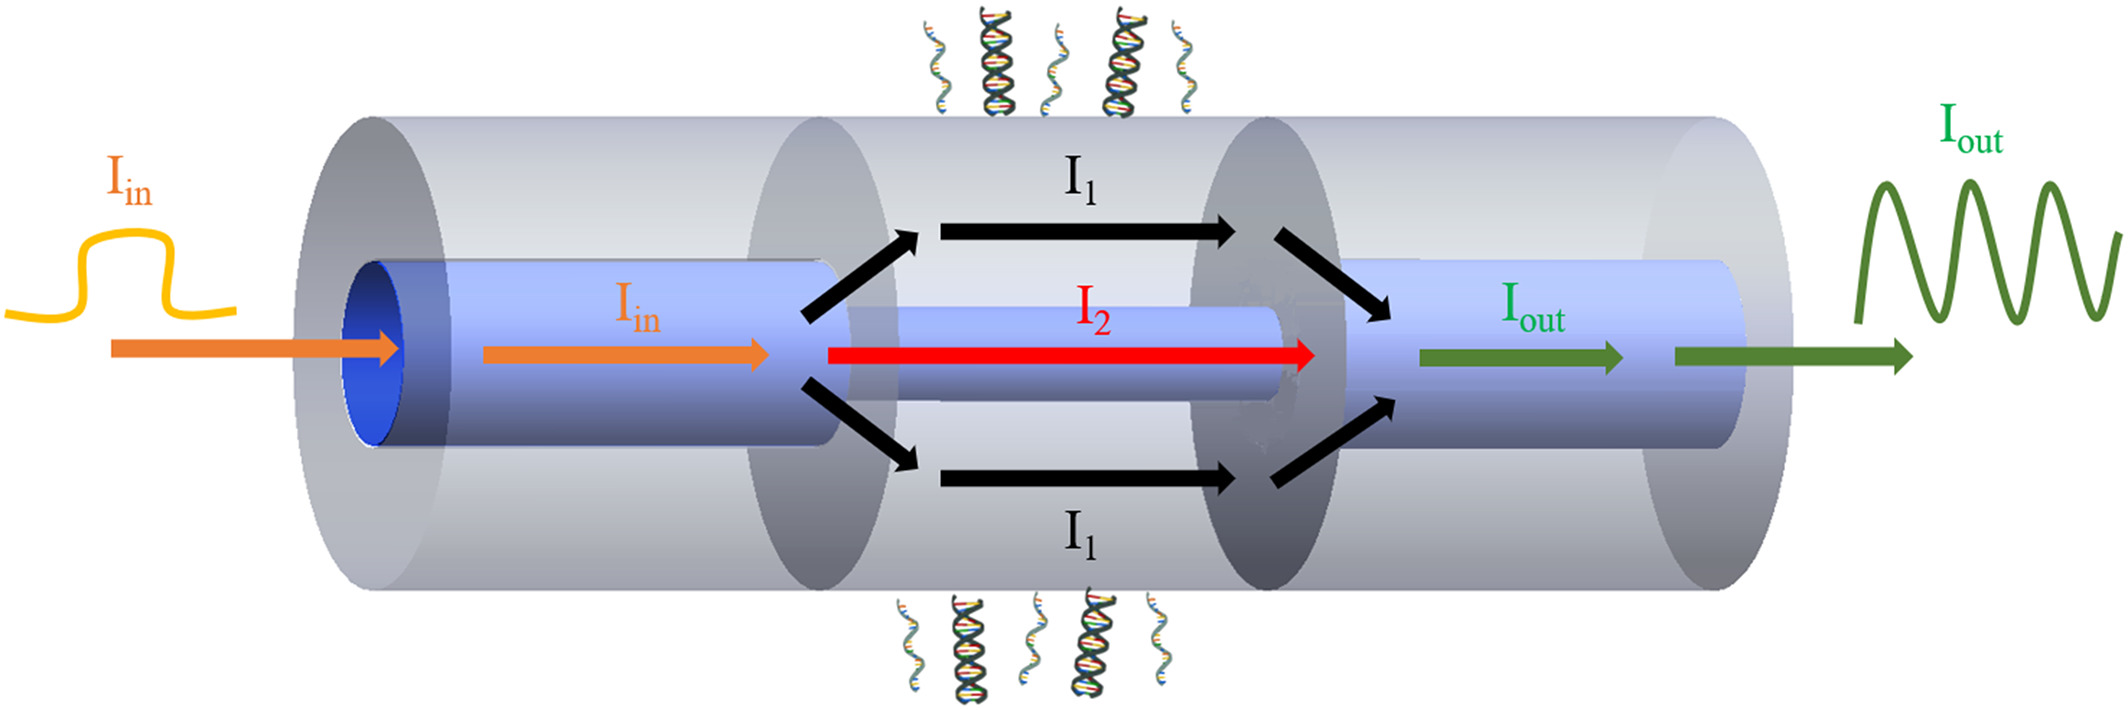
\includegraphics[width=0.45\textwidth]{attachments/figs.2.1.jpg}
            }
            \subfloat[Biosensors based on Michelson interferometer]{\label{fig.2.2}
            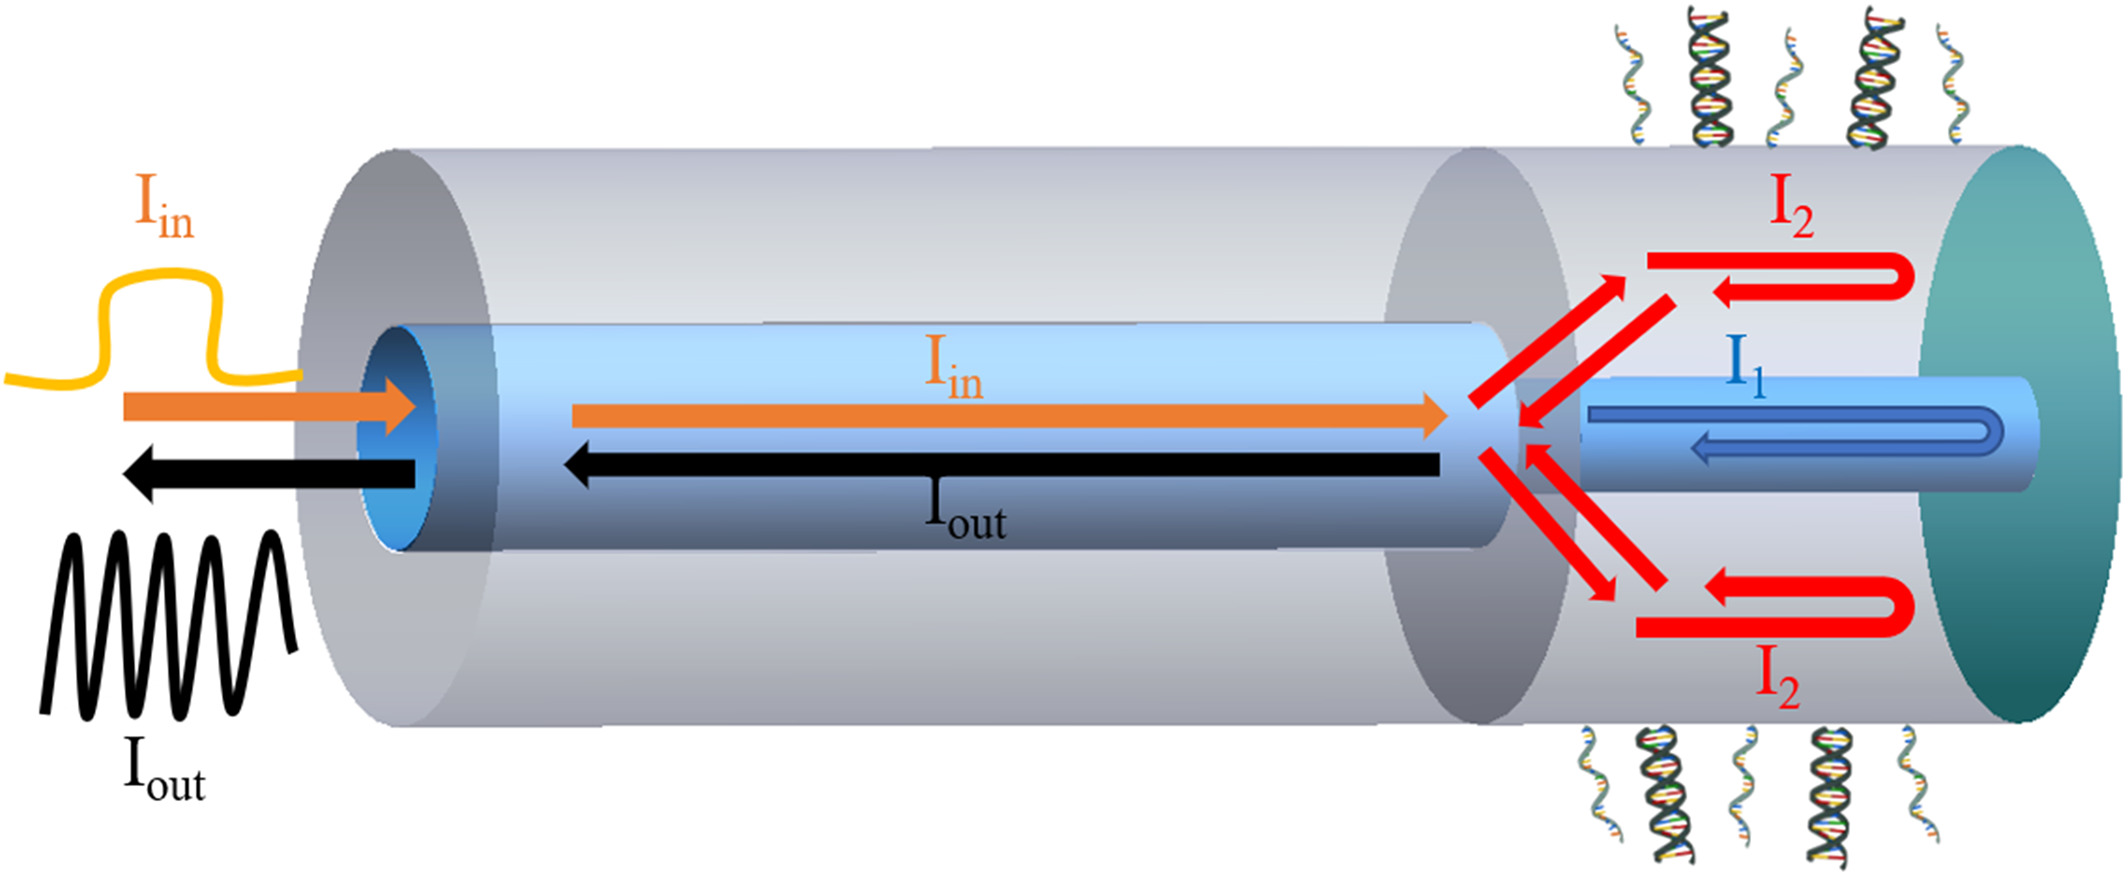
\includegraphics[width=0.45\textwidth]{attachments/figs.2.2.jpg}
            }
    
            \subfloat[Biosensors based on Sagnac interferometer]{\label{fig.2.3}
            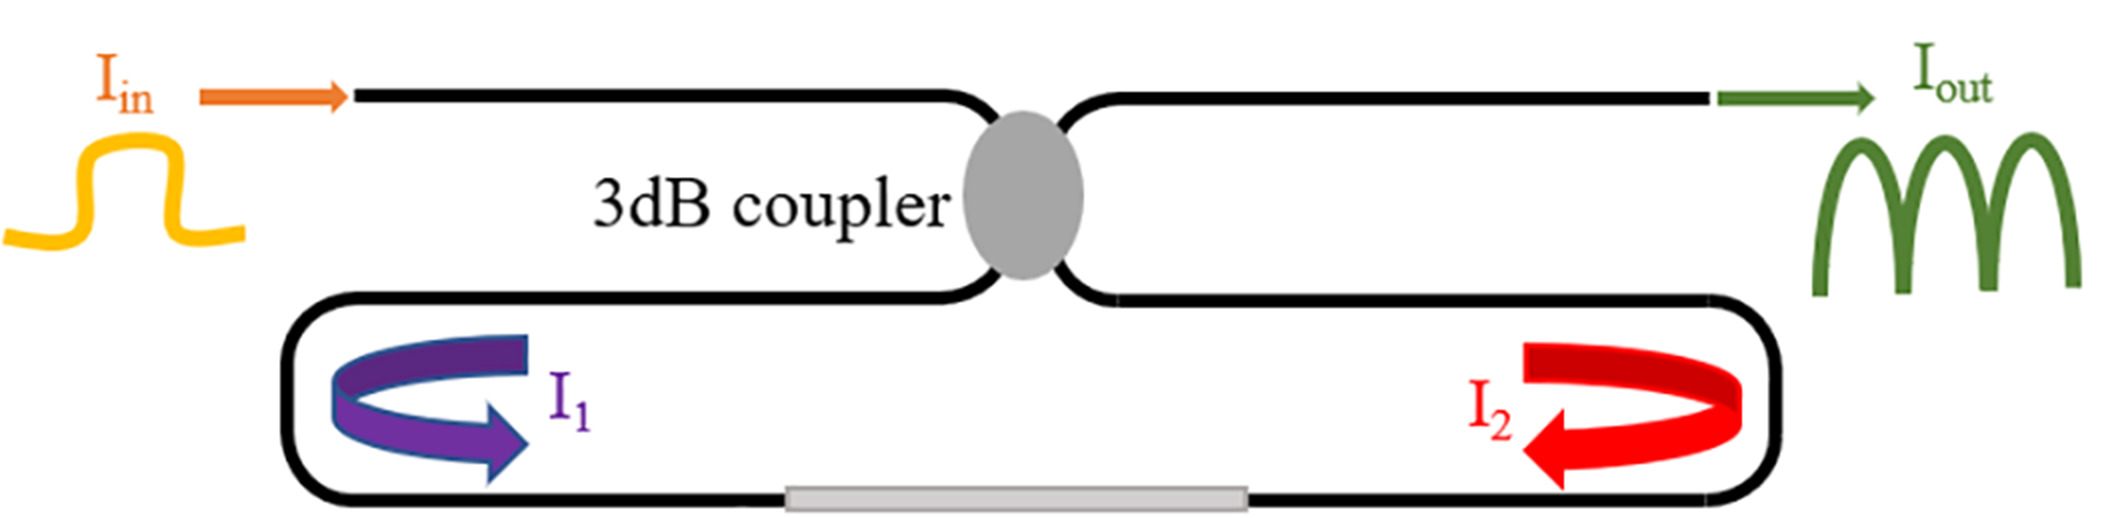
\includegraphics[width=0.45\textwidth]{attachments/figs.2.3.jpg}
            }
            \subfloat[Biosensors based on Fabry-Perot interferometer]{\label{fig.2.4}
            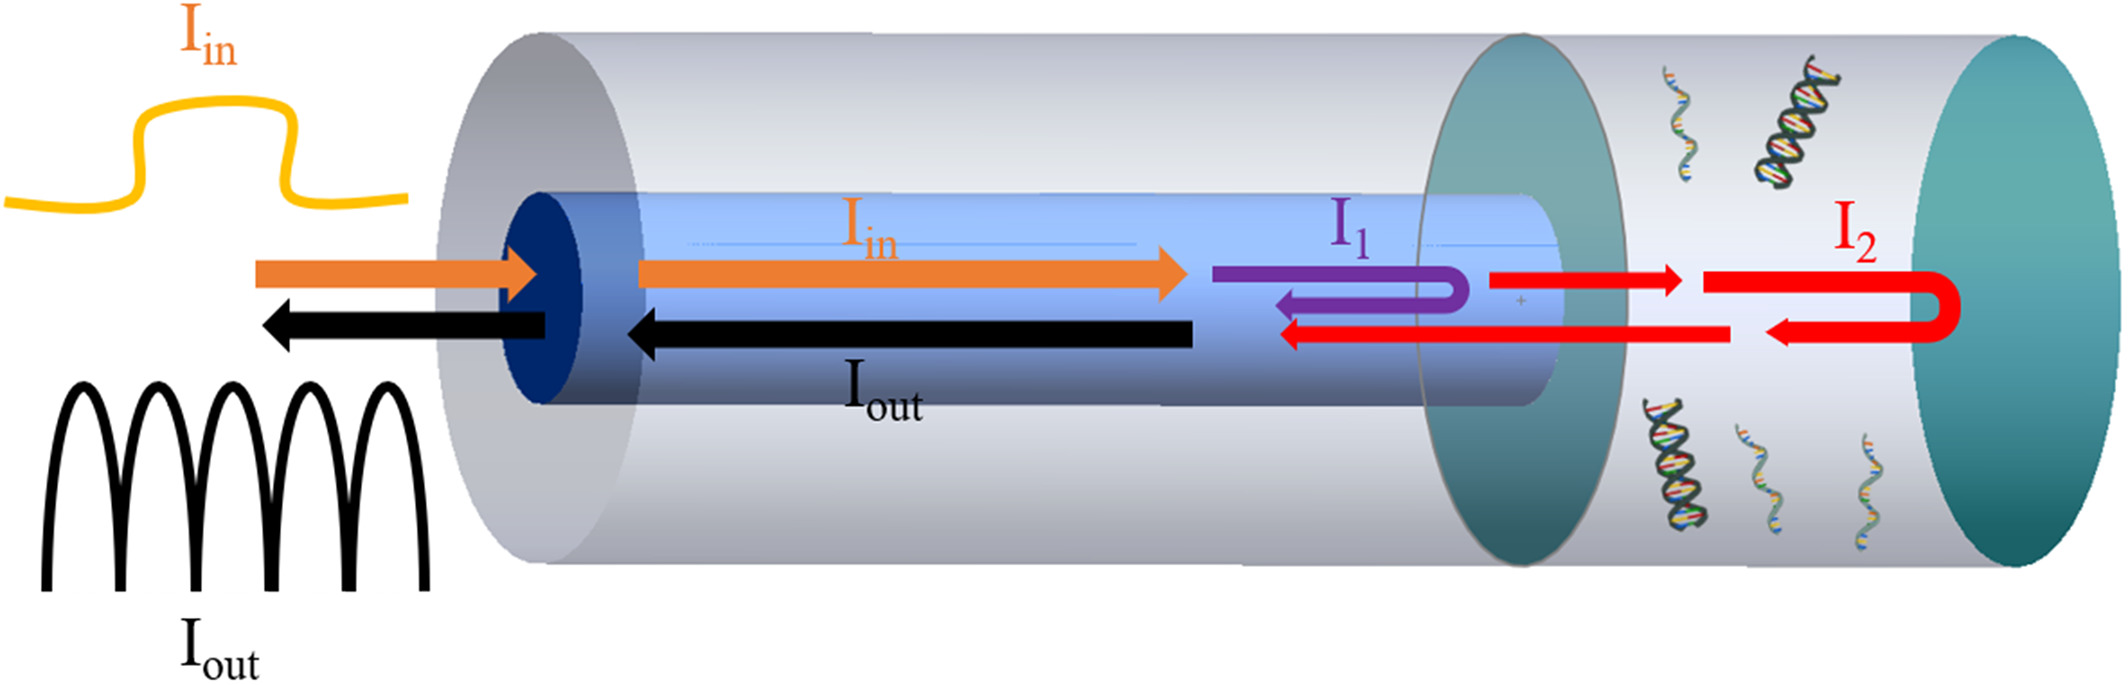
\includegraphics[width=0.45\textwidth]{attachments/figs.2.4.jpg}
            }
            \caption{\textbf{Fiber-based biosensor}}
        \end{figure}
    
    \section{Exp.3 Impact of transmission in a fiber on the polarization state}
    \subsection{Main parameters}
    \begin{table}[htbp]
        \centering
            \begin{tabular}{cc}
                \toprule
                Item &parameters  \\
                \midrule
                Fiber &$\phi \ 4 \mu m$ \\
                \bottomrule
            \end{tabular}
            \caption{\textbf{Parameters adopted in Exp. 3}}
            \label{tab.3.0}
    \end{table}	

    \subsection{Supplementary data and figure}
    \begin{enumerate}[label=\arabic*.]
        \item Fig. \ref{fig.3} Fluctuation of the light power after the fiber transmission
    \end{enumerate}
    \begin{figure}[htbp]
        \centering
        \subfloat[linearly polarized light]{\label{fig.3.1}
        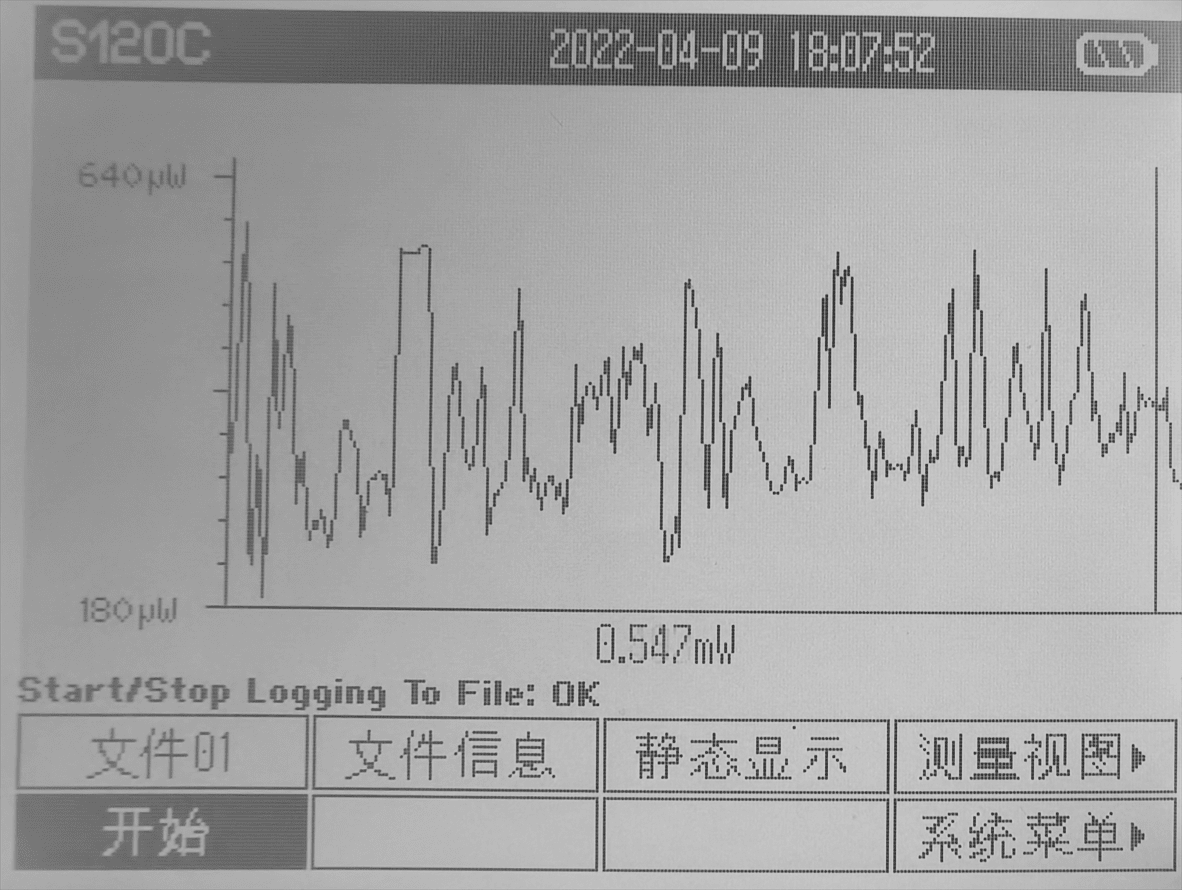
\includegraphics[width=0.3\textwidth]{attachments/figs.3.1.png}
        }
        \subfloat[Right-handed polarized light]{\label{fig.3.2}
        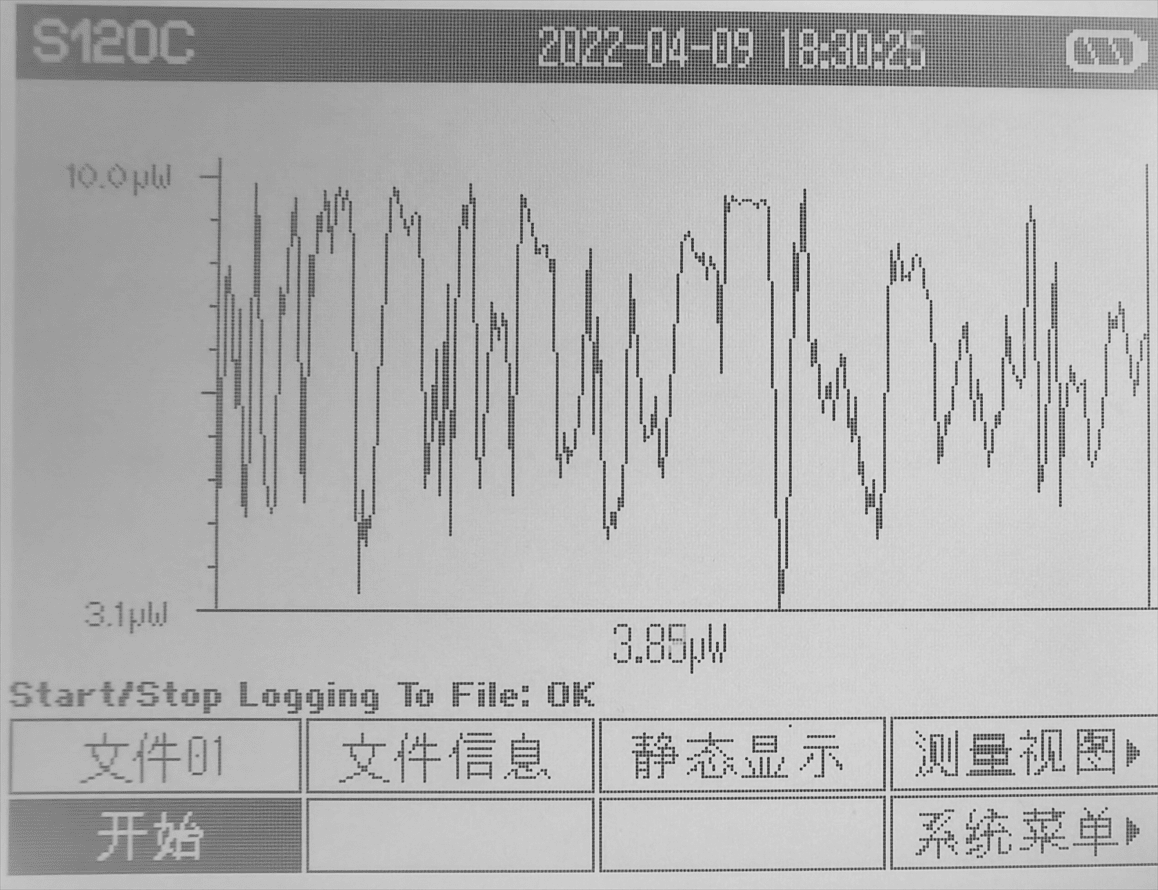
\includegraphics[width=0.3\textwidth]{attachments/figs.3.2.png}
        }

        \subfloat[Analyzer: x-axis]{\label{fig.3.3}
        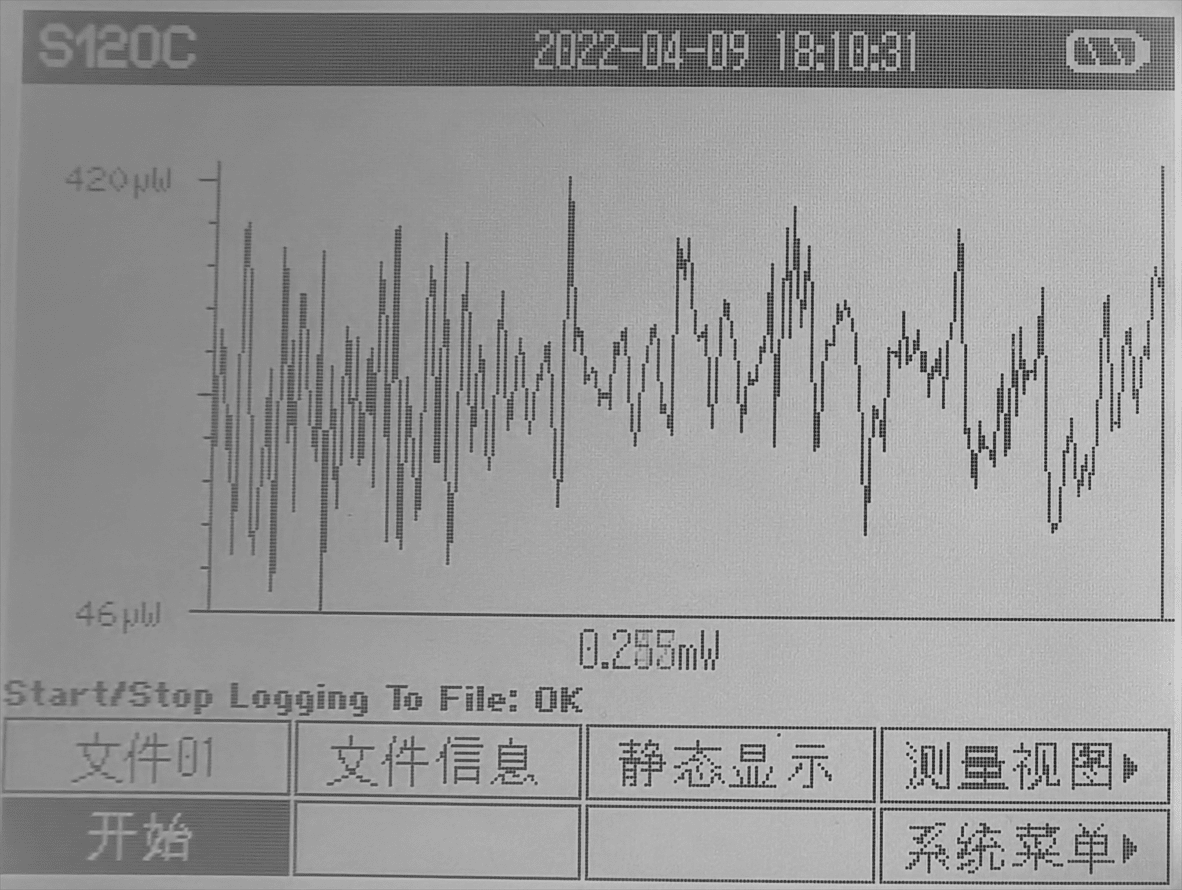
\includegraphics[width=0.3\textwidth]{attachments/figs.3.3.png}
        }
        \subfloat[Analyzer: y-axis]{\label{fig.3.4}
        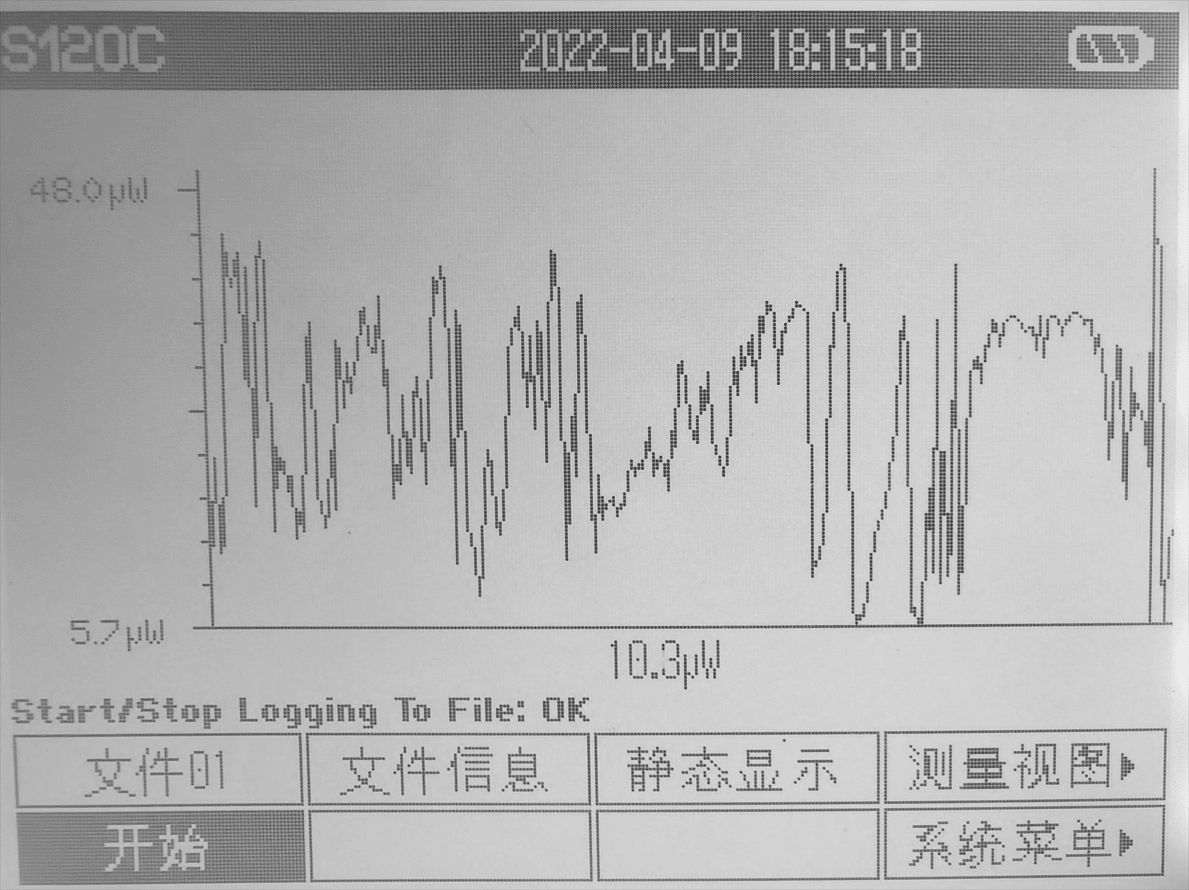
\includegraphics[width=0.3\textwidth]{attachments/figs.3.4.png}
        }
        \subfloat[Analyzer: $\frac{\pi}{4}$]{\label{fig.3.5}
        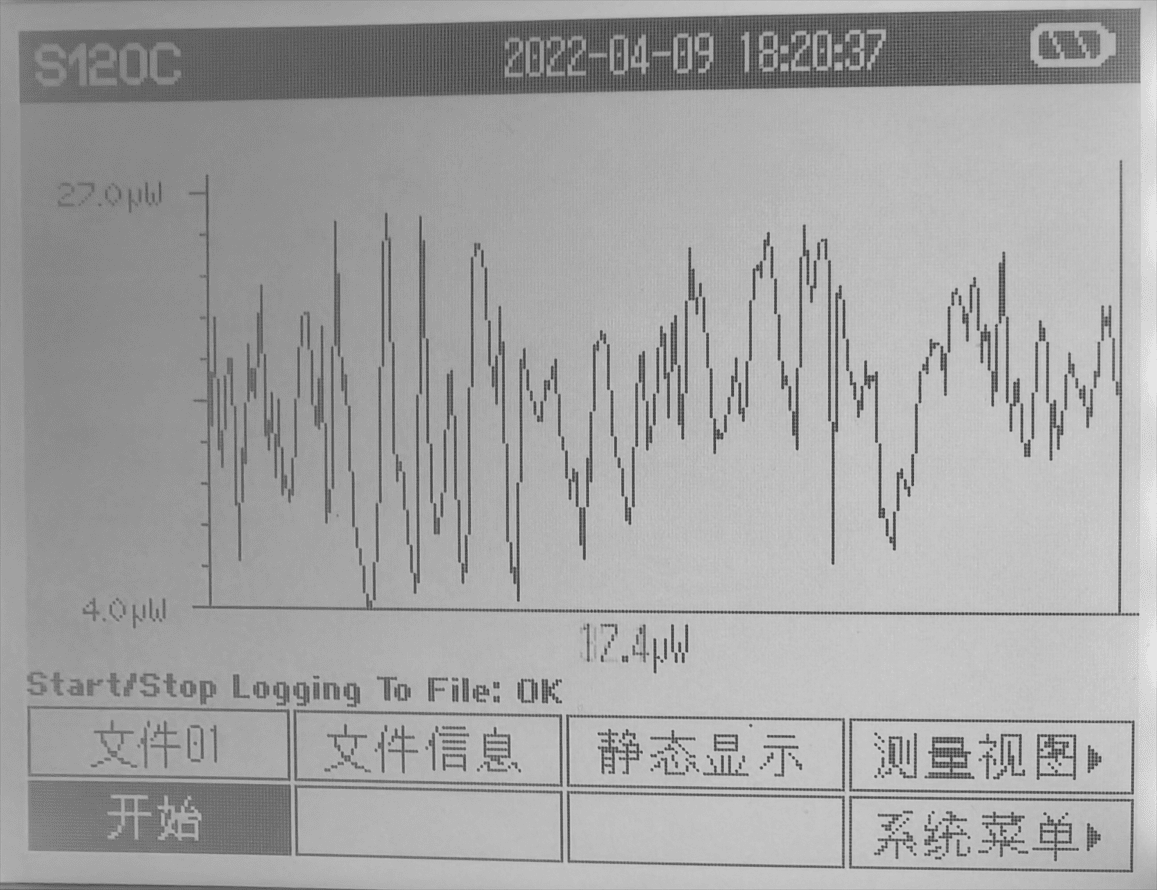
\includegraphics[width=0.3\textwidth]{attachments/figs.3.5.png}
        }
        \caption{\textbf{Fluctuation of the light power after the fiber transmission}}
        \label{fig.3}
    \end{figure}


    \subsection{Reflection question}
        \subsubsection{Analyze the experimental results and compare with the theoretical value. Analyze possible deviation.}
        This question hsa been discussed in details in the thesis.
        \subsubsection{Mechanism of the polarization-maintaining fibers.}
        Polarization-maintaining fiber is specialty fiber with a strong built-in birefringence (high-birefringence fiber or HIBI fiber). 
        Provided that the polarization of light launched into the fiber is aligned with one of the birefringent axes, this polarization state will be preserved even if the fiber is bent. 
        The propagation constants of the two polarization modes are significantly different due to the strong birefringence, 
        so that the relative phase of such copropagating modes rapidly drifts away. 
        Therefore, any disturbance along the fiber can effectively couple both modes only if it has a significant spatial Fourier component with a wavenumber which matches the difference of the propagation constants of the two polarization modes.
        
        A commonly used method for introducing strong birefringence is to include two (not necessarily cylindrical) stress rods of a modified glass composition (typically boron-doped glass, with a different degree of thermal expansion) in the preform on opposite sides of the core.
        (Fig. \ref{fig.4.1})
        
        \begin{figure}[htbp]
            \centering
            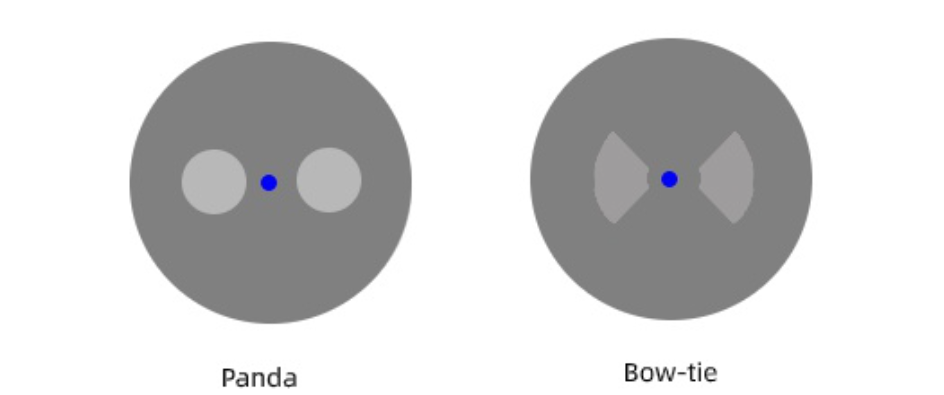
\includegraphics[width=0.4\textwidth]{attachments/figs.4.1.png}
            \caption{\textbf{Polarization-maintaining fiber}}
            \label{fig.4.1}
        \end{figure}

%end---------------------Supplementary Info---------------------------%

\section{Data and code availability}
Data and code are available at \url{https://github.com/Jeg-Vet/SYSU-PHY-EXP/tree/main/}

%%begin--------------------Reference------------------------%%
\printbibliography[title=Reference] 
%%end--------------------Reference------------------------%%
\end{document}